%%%%%%%%%%%%%%%%%%%%%%%%%%%%%%%%%%%%%%%%%%%%%%%%%%%%%%%%%%%%%%%%%%%%%%%%%%%%%%
%
% Section file included in main project file using \input{}
%
% Assumes that LaTeX2e macros and packages defined in cg_comp.sty are
%   available
%
%%%%%%%%%%%%%%%%%%%%%%%%%%%%%%%%%%%%%%%%%%%%%%%%%%%%%%%%%%%%%%%%%%%%%%%%%%%%%%

 \section{Classical Guitar Compensation\label{sct:comp}}

 \begin{table}[htbp]
  \centering
  \caption{\label{tbl:ej45_setbacks} Predicted setbacks for the D'Addario Pro-Arte Nylon Classical Guitar Strings -- Normal Tension (EJ45) on the Alhambra 8P classical guitar.}
  \begin{tabular}{cccc}
\toprule
String &  $\Delta S$ (mm) &  $\Delta N$ (mm) &  $\overline{\Delta \nu}_\text{rms}$ (cents) \\
\midrule
 J4501 &             2.16 &            -0.43 &                                        0.18 \\
 J4502 &             1.92 &            -0.31 &                                        0.15 \\
 J4503 &             4.36 &            -0.82 &                                        0.31 \\
 J4504 &             1.30 &            -0.19 &                                        0.13 \\
 J4505 &             1.94 &            -0.28 &                                        0.15 \\
 J4506 &             2.62 &            -0.35 &                                        0.16 \\
\bottomrule
\end{tabular}


 \end{table}%

 \begin{figure}
  \centering
  \begin{subfigure}[b]{0.45\textwidth}
   \centering
   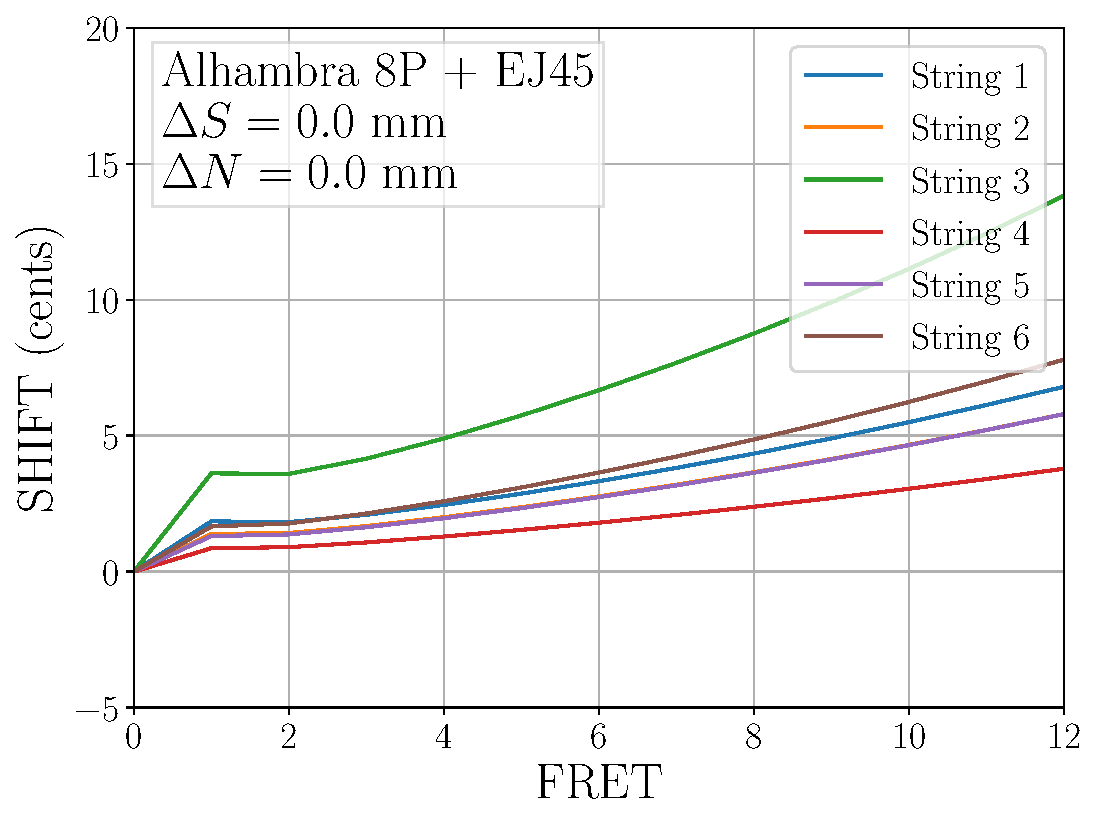
\includegraphics[width=3.25in]{figures/shift_alhambra8p_ej45_null}
   \caption{Uncompensated}
   \label{fig:shift_alhambra8p_ej45_null}
  \end{subfigure}
  \hspace{0.25in}
  \begin{subfigure}[b]{0.45\textwidth}
   \centering
   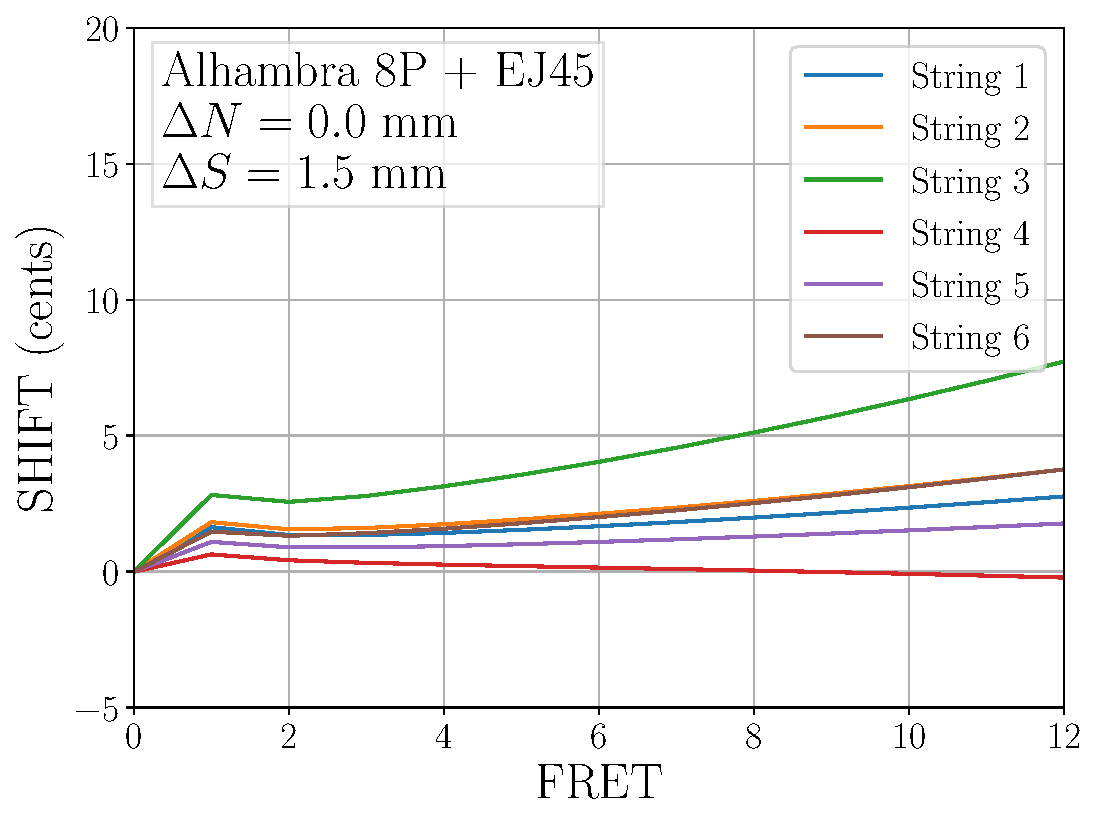
\includegraphics[width=3.25in]{figures/shift_alhambra8p_ej45_factory}
   \caption{Factory guitar}
   \label{fig:shift_alhambra8p_ej45_factory}
  \end{subfigure}
  \par\vspace{0.25in}
  \begin{subfigure}[b]{0.45\textwidth}
   \centering
   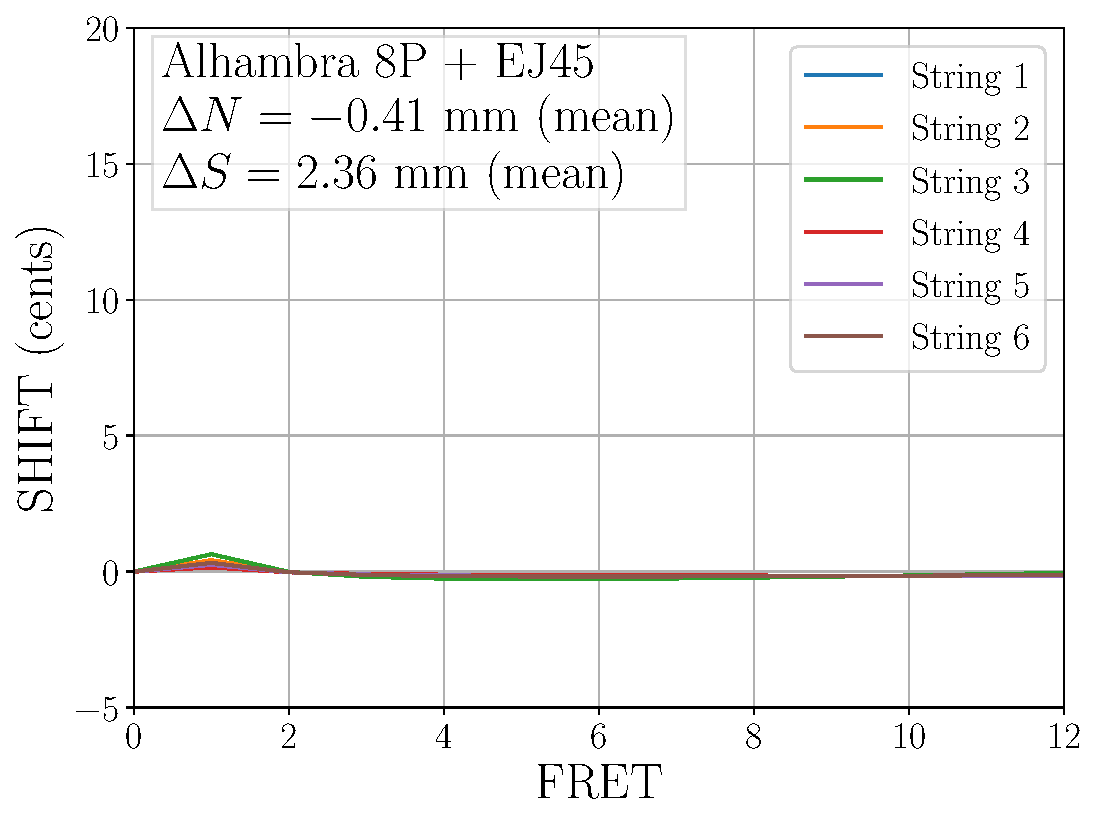
\includegraphics[width=3.25in]{figures/shift_alhambra8p_ej45_full}
   \caption{Full compensation}
   \label{fig:shift_alhambra8p_ej45_full}
  \end{subfigure}
  \hspace{0.25in}
  \begin{subfigure}[b]{0.45\textwidth}
   \centering
   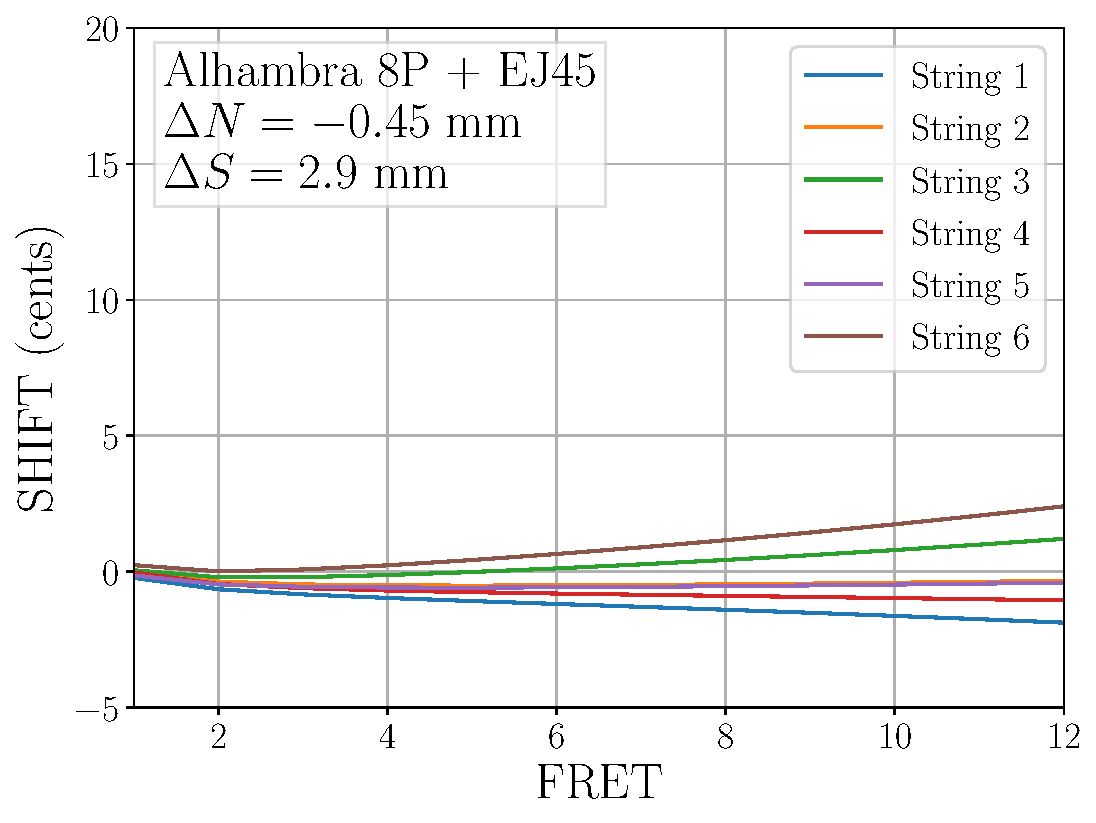
\includegraphics[width=3.25in]{figures/shift_alhambra8p_ej45_mean}
   \caption{Mean compensation}
   \label{fig:shift_alhambra8p_ej45_mean}
  \end{subfigure}
  \caption{\label{fig:compensation_alhambra8p_ej45} Frequency shift (in cents) for an Alhambra 8P guitar with D'Addario Pro-Arte Nylon Classical Guitar Strings -- Normal Tension (EJ45). Four different strategies of saddle and nut compensation are illustrated.}
 \end{figure}

